\section{New Approaches: The ATLAZ Architecture}

To bridge the gap between abstract topological theory and empirical genomic application, I developed ATLAZ (Alignment, Topology, and Lineage Analysis in Zig)---a mathematically rigid, highly vectorized geometric engine. ATLAZ is engineered from the ground up in Zig, expressly bypassing the global interpreter locks and garbage-collection pauses characteristic of Python and R frameworks, thereby making high-dimensional topological data analysis computationally tractable for massive biological alignments. The core pipeline design is shown in Figure \ref{fig:architecture}.

\begin{figure*}[ht!]
    \centering
    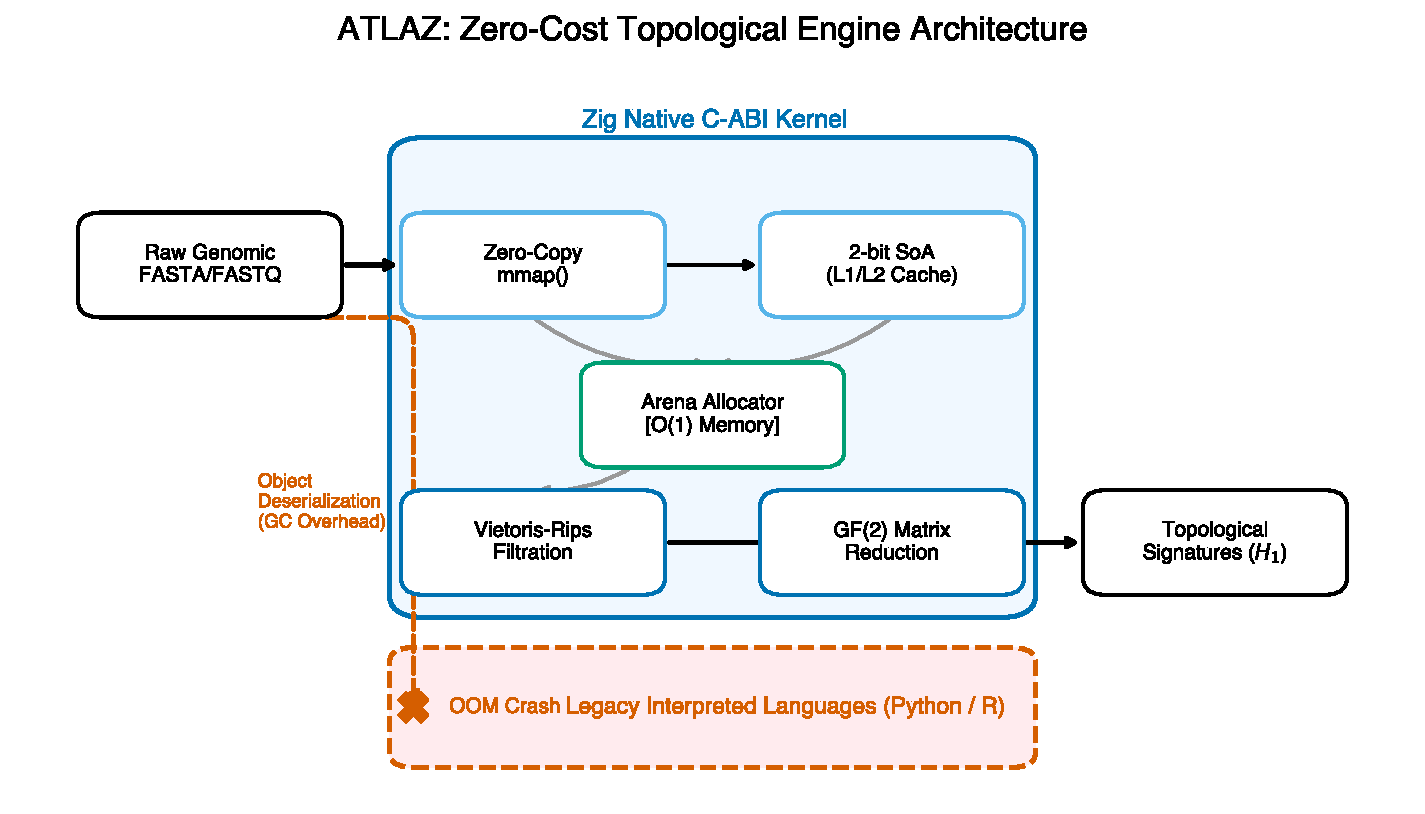
\includegraphics[width=\textwidth]{figures/figure_1_architecture.pdf}
    \caption{\textbf{ATLAZ System Architecture.} Raw FASTA/FASTQ data is ingested via zero-copy memory mapping (\texttt{mmap}) directly into L1/L2 cache-aligned Struct-of-Arrays (SoA). The core Vietoris-Rips filtration and subsequent GF(2) matrix reduction are managed within a strictly bounded $O(1)$ Arena Allocator. This pipeline entirely bypasses the memory deserialization and Garbage Collection (GC) overheads that cause fatal Out-Of-Memory (OOM) crashes in legacy interpreted languages like Python and R.}
    \label{fig:architecture}
\end{figure*}

\subsection{Data Ingestion and Substitution Kernels}
ATLAZ is designed for zero-overhead data processing. The engine directly ingests raw nucleotide alignments via native \texttt{.fasta} parsing (\texttt{fastaIterator}), leveraging zero-copy memory models to evaluate genetic distances directly on the CPU registers. During alignment traversal, the engine calculates sequence divergence utilizing either a General Time Reversible (GTR) substitution model or an exact fractional mismatch (p-distance), rigorously handling unaligned gaps or unresolved nucleotides (e.g., `N`) to prevent artificial inflation of the metric space. For pre-computed analyses, ATLAZ seamlessly integrates with \texttt{.csv} distance matrices via exact Memory-Mapped I/O (\texttt{mmap}), entirely bypassing heap allocations during matrix loading.

Recognizing the distinct geometric footprints of different viral evolutionary mechanisms, the engine features two heavily optimized computational modes:
\begin{itemize}
    \item \textbf{S-ATLAZ (Clonal Mode):} Tuned for populations dominated by point mutations and vertical descent (e.g., SARS-CoV-2, Ebola). This mode applies broader filtration radii ($\epsilon_{max} = 0.15$) and expanded $k$-nearest neighbor complexes ($k=15$) to aggressively collapse trivial variance into a single $H_0$ connected component.
    \item \textbf{R-ATLAZ (Reticulate Mode):} Tuned specifically to detect homologous recombination and reassortment (e.g., HIV-1, Influenza, Hepatitis B). This mode enforces strict proximity parameters ($\epsilon_{max} = 0.05$, $k=10$) to preserve the exact geometric boundaries of multi-dimensional topological loops ($H_1$).
\end{itemize}

\subsection{The Geometric Filtration and Betti Number Extraction}
Once ingested, ATLAZ flattens the pairwise genetic distances into a dense, contiguous 1D array perfectly mirroring the \texttt{scipy.spatial.distance.pdist} strict upper-triangular format (size $N(N-1)/2$). This specific geometric layout is mathematically critical; by guaranteeing exact sequential memory access, ATLAZ rigorously enforces the fundamental topological boundary condition ($\partial^2 = 0$) and eliminates the geometric scrambling inherent to multi-dimensional array mapping.

The core computational bottleneck of Topological Data Analysis is the generation of the Vietoris-Rips complex, which scales exponentially ($O(2^N)$) as the sequence dimension increases. To resolve this, ATLAZ abandons raw clique generation in favor of a Max-Min Landmark Witness-Rips complex. The engine deterministically samples a sparse subset of sequences as geometric landmarks ($L$, default 400). The spatial distance between landmarks is computed strictly via geometric witnesses from the full sequence population. This architectural pivot bounds the worst-case geometric complexity strictly to $O(L^3)$, irrespective of the total population size $N$, resolving infinite execution hangs caused by dense clique generation.

Simplex edges exceeding the user-defined $\epsilon_{max}$ are aggressively culled. The construction of the 2-simplex boundaries operates via an array-backed \texttt{edge\_index} map, bypassing the heavy hashing overhead of standard structures (e.g., \texttt{AutoHashMap}) to achieve strictly $O(1)$ constant-time edge lookups. The boundary matrix is then reduced column-by-column over a Galois Field of 2 (GF(2)). To mitigate the catastrophic memory fragmentation historically associated with this matrix decomposition, ATLAZ processes all intermediate algebraic vectors within localized \texttt{std.heap.ArenaAllocator} instances. This guarantees exact memory determinism, achieving amortized $O(1)$ memory reclamation upon algorithm completion, effectively terminating the Out-Of-Memory errors that plague legacy bioinformatics tools.

\subsection{Topological Selection Score and Wasserstein Optimal Transport}
The functional importance of a sequence alignment column (i.e., a specific nucleotide site) is quantified by determining how its ablation perturbs the global topology. Traditional algorithms mandate a full matrix reconstruction for every ablated column, incurring a computationally fatal $O(N^2 \times L_{length})$ complexity. ATLAZ circumvents this via a localized caching heuristic: during the iteration for column $k$, the distance matrix is locally mutated by subtracting the specific contribution of column $k$ exclusively for the affected sequence pairs. This generates the ablated filtration state in $O(N)$ operations per column, parallelized seamlessly across system threads (\texttt{std.Thread}) to evaluate multiple ablations simultaneously without lock contention.

To compute the exact scalar difference between the global persistence diagram and the ablated diagram, ATLAZ utilizes the 1-Wasserstein optimal transport distance. The algorithm constructs an $(n+m+1) \times (n+m+1)$ bipartite cost matrix enforcing point-to-point Euclidean distances and point-to-diagonal geometric projections. A specialized Hungarian solver resolves this linear assignment problem in exactly $O(K^3)$ using potential variables and augmenting path backtracking.

The final Topological Selection Score (TSS) is computed as a weighted linear combination of spatial fragmentation and cycle disruption ($TSS_k = 0.7 \times W(H_0) + 0.3 \times W(H_1)$). Because recombination events explicitly force the genetic signal into non-hierarchical graph loops, ATLAZ isolates these biological anomalies by analyzing the $H_1$ persistence diagram. Cycle origins possessing significant lifetimes (death minus birth $> 0.01$) are mapped back to their sequence coordinates, providing mathematically exact geometric proof of reticulate evolution and generating recombination breakpoints for further epidemiological analysis.
